\begin{frame}[label=ears]
    \frametitle{Analogy: Ears as Interferometric Arrays}
    You locate sounds by comparing what each ear hears:  
    \begin{columns}
        \begin{column}{0.2\textwidth}
            \small \textit{A sound from your right hits your right ear first}
        \end{column}
        \begin{column}{0.4\textwidth}
            \centering
            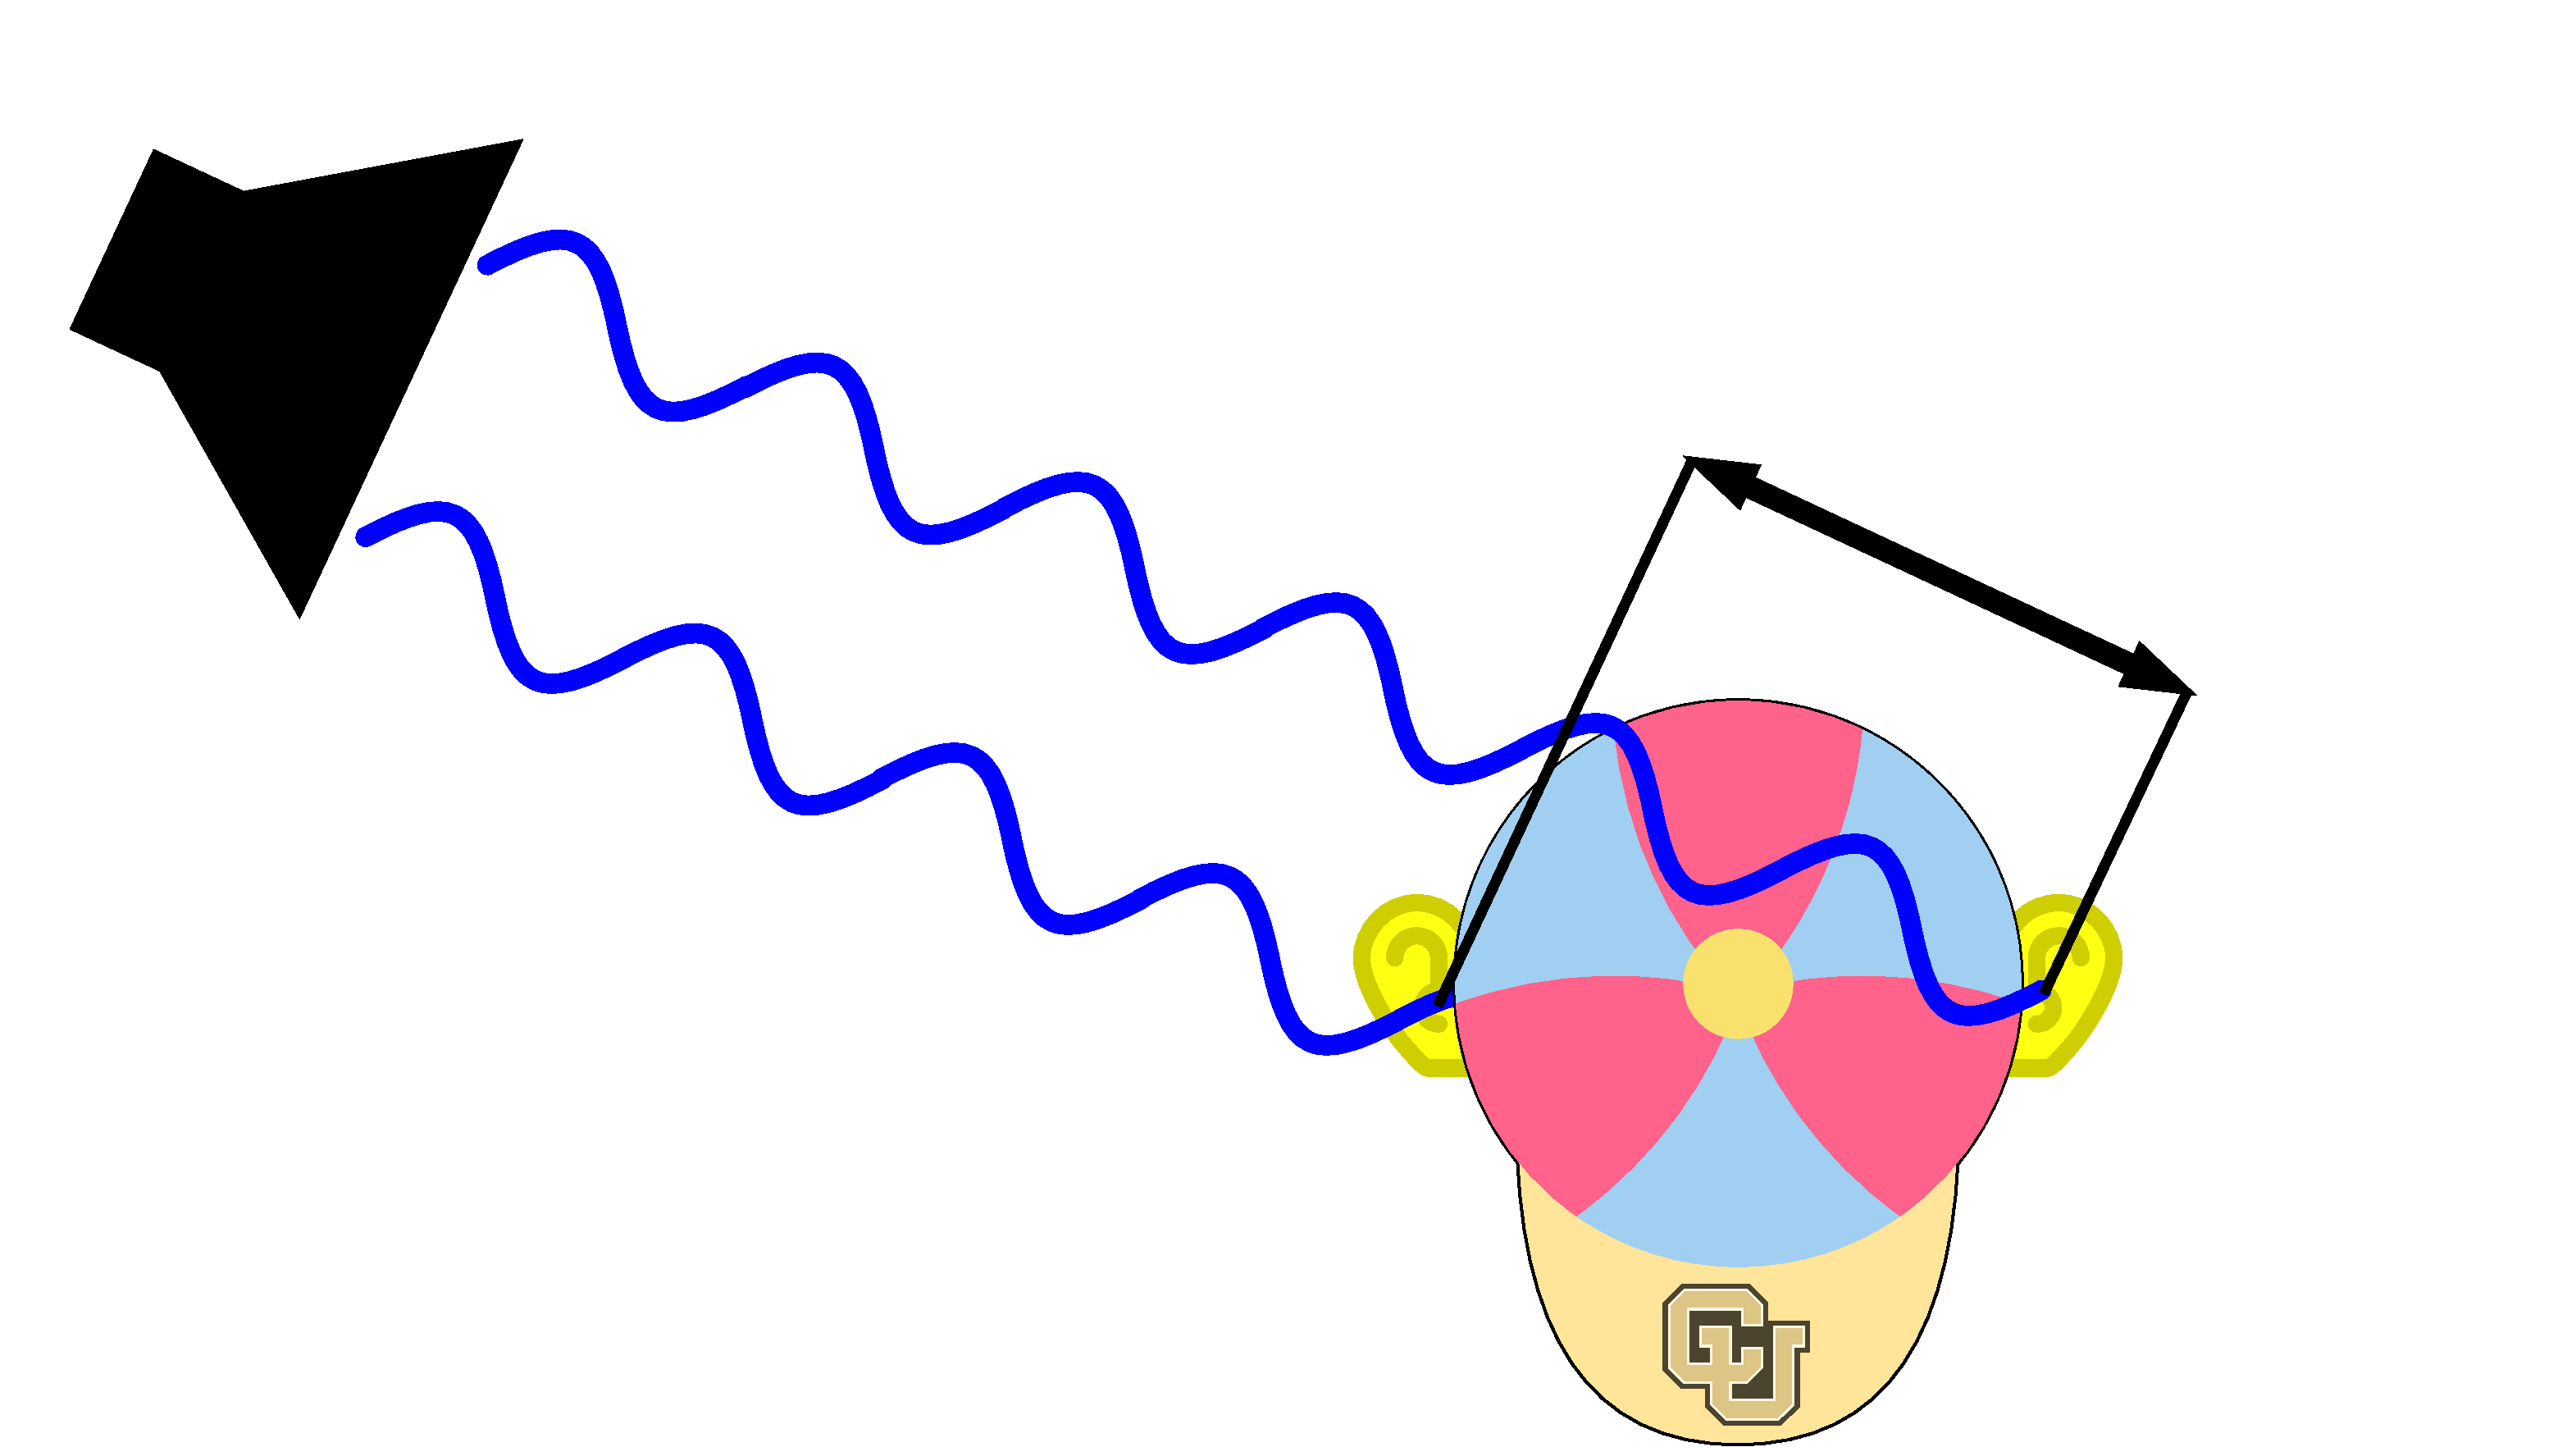
\includegraphics[scale=0.1]{img/ears_left.pdf}
        \end{column}
        \begin{column}{0.2\textwidth}
            \centering
            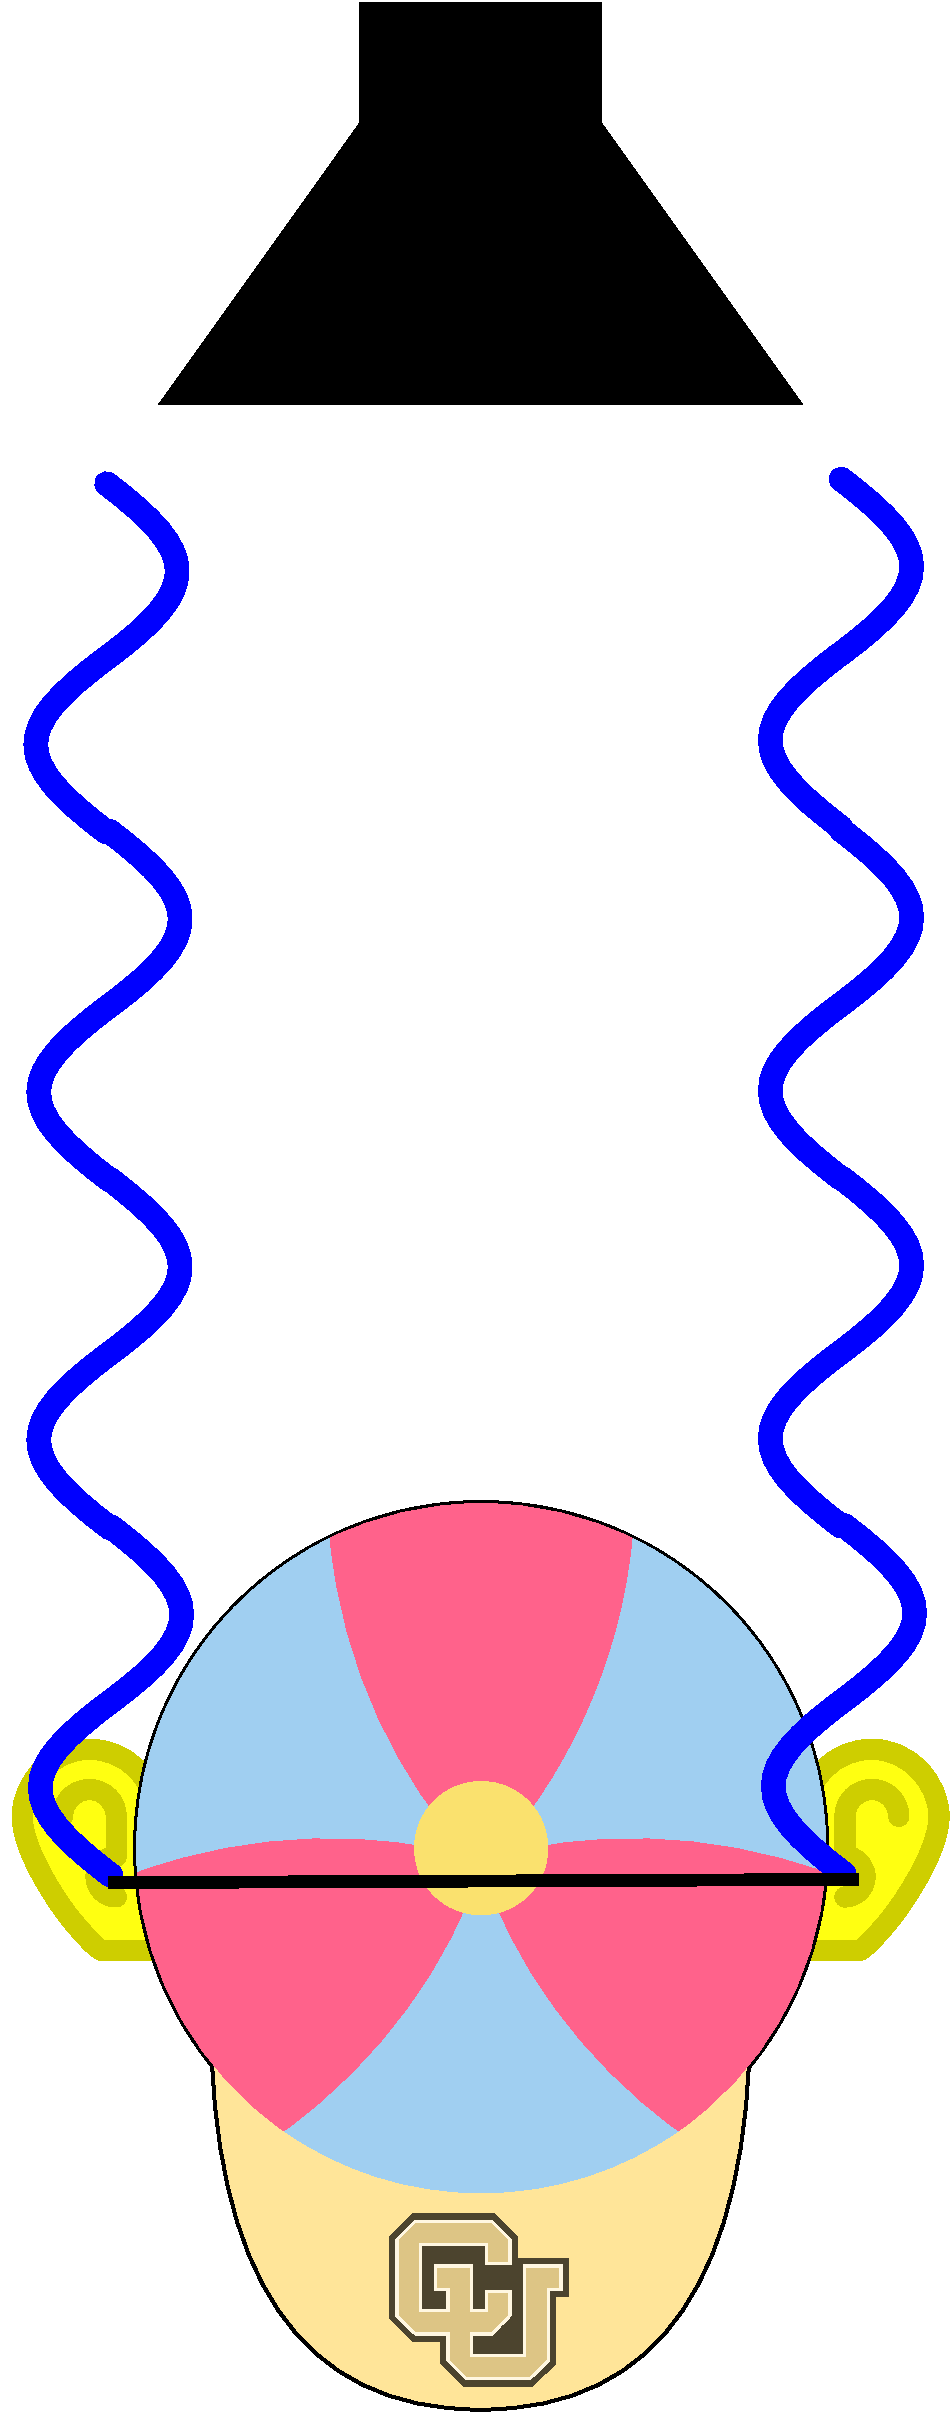
\includegraphics[scale=0.1]{img/ears_behind.pdf}
        \end{column}
        \begin{column}{0.2\textwidth}
            \small \textit{A sound from behind arrives at both ears simultaneously}
        \end{column}
    \end{columns}

    This is analogous to interferometry! 
\end{frame}
